\documentclass[dvipsnames,tikz]{standalone}
\usepackage{amsmath}
\usepackage{xcolor}
\usepackage{tikz}
\usetikzlibrary{calc}
\usetikzlibrary{decorations.pathreplacing,calligraphy,3d}
\usetikzlibrary{positioning}

\tikzset{main/.style={draw=black, circle, color=black}}

\begin{document}
	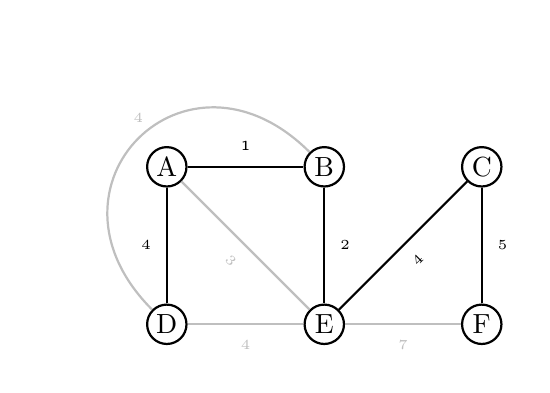
\begin{tikzpicture}[node distance={20mm}, thick,inner sep=0pt,minimum size=5mm] 
		\node[main] (A) {A}; 
		\node[main] (B) [right of=A] {B};
		\node[main] (C) [right of=B] {C};
		\node[main] (D) [below of=A] {D};
		\node[main] (E) [below of=B] {E};
		\node[main] (F) [below of=C] {F};
		
		\begin{scope}[font=\tiny]
			\draw[main] (A) -- node[midway, above] {1} (B);
			\draw[main] (B) -- node[midway, right] {2} (E);
			\draw[main] (A) -- node[midway, left] {4} (D);
			\draw[color=lightgray] (D) -- node[midway, below] {4} (E);
			\draw[main] (A) -- node[midway, above] {1} (B);
			\draw[main] (E) -- node[midway, below, sloped] {4} (C);
			\draw[main] (C) -- node[midway, right] {5} (F);
			\draw[color=lightgray] (E) -- node[midway, below] {7} (F);
			\draw[color=lightgray] (A) -- node[midway, below, sloped] {3} (E);
			\draw[color=lightgray] (D) to [out=135,in=135,looseness=2] node[midway, above] {4} (B);
		\end{scope}
	\end{tikzpicture} 
\end{document}